\section{Szczegóły implementacyjne}
\label{sec:szczegoly-implementacyjne}

\subsection{Wykorzystane technologie oraz narzędzia programistyczne}
Projekt jest realizowany na platformie FPGA, więc musi zostać napisany w języku opisu sprzętu. Wykorzystany został język VHDL, ze względu na jego silną kontrolę typów, która pozwala na wczesne wykrywanie niektórych błędów podczas kompilacji, co okazało się bardzo pomocne podczas implementowania modułów AES.

Środowiskiem programistycznym, które zostało wykorzystane do realizacji tego projektu jest Altera Quartus Prime 15.1 Lite Edition. Taki wybór był podyktowany faktem, że wykorzystana w projekcie płytka Terasic DE1-SOC wyposażona jest w układ FPGA firmy Altera, a Quartus jest jedynym środowiskiem przeznaczonym do tworzenia oprogramowania dla układów FPGA tej firmy.

Do realizacji projektu zostało wykorzystane narzędzie QSys, które wchodzi w skład środowiska Quartus oraz służy do integracji zasobów dostępnych na płytce w projekcie, np. HPS, RAM. Pozwala również na konfigurację tych komponentów, co ma kluczowe znaczenie dla wykorzystania znajdującego się na płytce konwertera USB UART (patrz rozdział \ref{sec:uart-qsys}).

Do przygotowania karty SD wykorzystane zostało środowisko Altera SoC FPGA Embedded Design Suite 15.1, które zawiera narzędzia programistyczne przeznaczone do tworzenia projektów korzystających zarówno z programowalnej części FPGA jak i procesora HPS. Użyte zostało narzędzie \textit{bsp-editor}, które posłużyło do wygenerowania preloadera (patrz rozdział \ref{sec:uart-preloader-gen}).

Testy implementowanych komponentów były realizowane jako symulacje funkcyjne przy pomocy narzędzi wchodzących w skład środowiska programistycznego Quartus.


\subsection{Przygotowanie oraz konfiguracja projektu}

Terasic -- producent wykorzystanej w tym projekcie płytki płytki DE1-SOC -- opracował i udostępnił na płycie CD dołączonej do zestawu \cite{??} projekt bazowy GHRD (ang. \textit{Golden Hardware Reference Design}). Jest to projekt skonfigurowany do poprawnego działania z płytką DE1-SOC, w którym ustawione są m.in.
\begin{itemize}[noitemsep]
\item model układu FPGA znajdującego się na płytce
\item konfiguracja pinów
\item podstawowe ograniczenia czasowe układu
\item projekt QSys reprezentujący zintegrowany procesor HPS (ang. \textit{Hard Processor System})
\item główny plik projektu (ang. \textit{top-level entity}) wraz z dodanym komponentem reprezentującym HPS
\end{itemize}
Projekt GHRG zawiera podstawowe ustawienia, więc umożliwia programiście skrócenie etapu konfiguracji projektu oraz szybkie rozpoczęcie pracy nad projektowanym układem. Bazą dla tego projektu był GHRD.

Do konwersji sygnału USB do UART wykorzystany został znajdujący się na płytce Terasic DE1-SOC układ firmy FTDI. Jego sygnały nie są jednak podłączone bezpośrednio do programowalnej części układu FPGA, lecz do zintegrowanego procesora ARM. Aby uzyskać dostęp do jego sygnałów z FPGA należy odpowiednio dostosować projekt oraz stworzyć i wgrać na kartę SD preloader, który podczas uruchamiania płytki przestawi piny UART w odpowiedni tryb działania oraz określi ich kierunek.

\subsubsection{Konfiguracja pinów UART}
\label{sec:uart-qsys}
Aby skonfigurować projekt tak, aby układ FPGA miał dostęp do sygnałów UART konwertera USB UART podłączonych do HPS, należy wykonać następujące czynności \cite{altera-youtube-loanerio, altera-forum-fgga-hps-access, altera-forum-cant-rx}:

\begin{enumerate}
\item Otworzyć w edytorze QSys plik \textit{soc-system.qsys}
\item Wybrać komponent \textit{hps\_0} oraz w zakładce \textit{Peripheral Pins} dokonać zmian:
	\begin{itemize}[noitemsep,nolistsep]
	\item Zmienić wartość \textit{UART0 pin} na \textit{FPGA}
	\item Zmienić wartość \textit{UART0 mode} na \textit{Full}
	\item Zaznaczyć \textit{LOANIO 49} oraz \textit{LOANIO 50}
	\end{itemize}
\item Zapisać zmiany, oraz wygenerować kod VHDL klikając przycisk \textit{Generate HDL...}.
\item W głównym pliku projektu (ang. \textit{Top-Level Entity}) zmodyfikować komponent \textit{soc-system} tak, aby był zgodny z jego na nowo wygenerowaną wersją.
\item Przypisać wartość \textit{'1'} sygnałom:
	\begin{itemize}[noitemsep,nolistsep]
	\item \textit{hps\_0\_uart0\_cts}
	\item \textit{hps\_0\_uart0\_dsr}
	\item \textit{hps\_0\_uart0\_dcd}
	\item \textit{hps\_0\_uart0\_ri}
	\item \textit{hps\_0\_uart0\_rxd}
	\end{itemize}
\item Sygnał \textit{hps\_0\_hps\_io\_hps\_io\_gpio\_inst\_LOANIO49} przypisać do pinu \textit{HPS\_UART\_RX}.
\item Sygnał \textit{hps\_0\_hps\_io\_hps\_io\_gpio\_inst\_LOANIO50} przypisać do pinu \textit{HPS\_UART\_TX}.
\item Wektor sygnałów \textit{hps\_0\_h2f\_loan\_io\_oe} określa kierunek pinów pinów \textit{LOANIO}.
	\begin{itemize}[noitemsep,nolistsep]
	\item Do sygnału \textit{hps\_0\_h2f\_loan\_io\_oe(49)}, który odpowiada sygnałowi UART RX przypisać wartość \textit{'1'}, co odpowiada kierunkowi \textit{out}.
	\item Do sygnału \textit{hps\_0\_h2f\_loan\_io\_oe(50)}, który odpowiada sygnałowi UART TX przypisać wartość \textit{'0'}, co odpowiada kierunkowi \textit{in}.
	\end{itemize}
\end{enumerate}

Powyższe zmiany spowodują, że:
\begin{itemize}[noitemsep]
\item Sygnał \textit{hps\_0\_h2f\_loan\_io\_out(49)} będzie odpowiadał sygnałowi UART RX oraz będzie poprawnie połączony z konwerterem USB-UART firmy FTDI.
\item Sygnał \textit{hps\_0\_h2f\_loan\_io\_out(50)} będzie odpowiadał sygnałowi UART TX oraz będzie poprawnie połączony z konwerterem USB-UART firmy FTDI
\end{itemize}

\subsubsection{Przygotowanie preloadera}
\label{sec:uart-preloader-gen}
Aby przy starcie płytki piny UART zostały poprawnie połączone z układem FPGA należy z plików powstałych w wyniku kompilacji projektu wygenerować preloader. Aby to zrobić posłużyłem się narzędziem \textit{bsp-editor} będącym częścią oprogramowania Quartus, zgodnie z instrukcją znalezioną w internecie \cite{rocketboards-preloader}.

\subsubsection{Skrypt startowy programujący układ FPGA}
Aby automatycznie zaprogramować układ FPGA podczas startu urządzenia stworzyłem skrypt, który będzie się wykonywał w fazie U-Boot \cite{rocketboards-uboot-script}.
\begin{lstlisting}
fatload mmc 0:1 $fpgadata soc_system.rbf;
fpga load 0 $fpgadata $filesize;
\end{lstlisting}
Do programowania układu FPGA przy pomocy skryptu potrzebny jest plik konfiguracyjny w formacie \textit{.rbf}. Można go stworzyć konwertując przy pomocy środowiska Quartus plik \textit{.sof} powstały w wyniku kompilacji projektu \cite{rocketboards-sof-to-rfb}. Użyłem trybu programowania \textit{Fast Passive Parallel X16}, któremu odpowiada ustawienie przełączników MSEL[0:4] znajdujących się na płytce na wartość 00100.

\subsubsection{Przygotowanie karty SD}
Najłatwiejszym sposobem na stworzenie karty SD zawierającej potrzebne pliki jest modyfikacja dostarczonych na płycie CD do płytki Terasic DE1-SOC przykładowych obrazów. Lista kroków realizujących to zadanie przy użyciu komputera z systemem operacyjnym Linux \cite{rocketboards-booting-prebuild, rocketboards-updating-sd}:
\begin{enumerate}
\item Po włożeniu karty SD do czytnika należy określić jej ścieżkę w systemie operacyjnym, najlepiej analizując plik \textit{/proc/partitions}. Załóżmy, że ścieżką karty jest \textit{/dev/sdx}.
\begin{lstlisting}
  $ cat /proc/partitions
\end{lstlisting}

\item Wgrać dostarczony przez producenta obraz \textit{DE1\_SoC\_SD.img} na kartę SD.
\begin{lstlisting}
  $ sudo dd if=DE1\_SoC\_SD.img of=/dev/sdx bs=1M
  $ sudo sync
\end{lstlisting}

\item Zastąpić domyślny preloader
\begin{lstlisting}
  $ sudo dd if=preloader-mkpimage.bin of=/dev/sde3 bs=64k seek=0
  $ sudo sync
\end{lstlisting}

\item Wgrać skrypt U-Boot oraz plik zawierający konfigurację układu FPGA na partycję FAT \textit{/dev/sdx1} dowolnym sposobem (np. korzystając z systemowego eksploratora plików).
\end{enumerate}

Aby przy starcie płytki programowanie FPGA przebiegło pomyślnie, należy umieścić kartę SD w czytniku oraz ustawić przełączniki MSEL[4:0] w pozycji 00100.

\subsubsection{Główny zegar}
\label{clk-16}
Główny zegar \textit{CLK\_16}, którym taktowany będzie projektowany układ ma częstotliwość
\begin{equation}
f_{CLK\_16} = 16 * UART\_BAUD\_RATE
\end{equation}
gdzie \textit{UART\_BAUD\_RATE} jest szybkością transmisji sygnału UART wyrażoną w baudach, która dla tego projektu wynosi 115200 baudów. Taka wartość podyktowana jest faktem, że częstą praktyką interpretacji sygnału UART, jest jego próbkowanie z częstotliwością 16 razy szybszą niż częstotliwość zmian sygnału.

Częstotliwość zegara \textit{CLK\_16} jest o wiele niższa niż dostępny w układzie FPGA zegar o częstotliwości 50MHz. Pozwoliło to na uzyskanie żądanej częstotliwości przy pomocy prostego dzielnika częstotliwości.

\begin{figure}[!h]
	\begin{lstlisting}[style=vhdl, caption=Dzielnik częstotliwości, captionpos=b]
	entity uart_prescaler is
		port (
			clk_in  : in  std_logic;  --50MHz
			clk_out : out std_logic); --16 * 115200Hz
	end uart_prescaler;
	
	architecture uart_prescaler_impl of uart_prescaler is
		signal clk : std_logic := '0';
	begin
		clk_out <= clk;
		
		process (clk_in) 
			variable counter : Integer range 0 to 13 := 0;
		begin	
			if(rising_edge(clk_in)) then
				case counter is
					when 13 =>
						clk <= not clk;
						counter := 0;
					when others =>
						counter := counter + 1;
				end case;
			end if;
		end process;
	end uart_prescaler_impl;
	\end{lstlisting}
\end{figure}

Układ jest wyzwalany rosnącymi zboczami zegara \textit{CLK\_16}. Jeśli akcja mająca miejsce w danym rosnącym zboczu zależy od wartości innego sygnału, to ma on stałą wartość co najmniej od poprzedzającego do następnego zbocza malejącego.


\subsubsection{Synchronizacja sygnału UART RX}
\label{uart-sync}
Sygnał UART RX pochodzi z peryferyjnego konwertera USB-UART firmy FTDI, który jest w domenie innego zegara. Powoduje to, że w momencie wystąpienia zbocz rosnących lub malejących głównego zegara, sygnał RX może nie mieć dobrze określonej wartości (np. również być w trakcie zbocza). Może to prowadzić do wystąpienia stanów metastabilnych \cite{altera-metastability} i w efekcie doprowadzić do niedeterministycznego działania układu. Aby temu zapobiec zsynchronizowałem sygnał RX, prowadząc go przez dwa przerzutniki typu D \cite{altera-metastability, 2ff-synchronization} wyzwalane głównym zegarem. Jest to standardowa technika, która powoduje drastyczne zmniejszenie prawdopodobieństwa wystąpienia stanów metastabilnych z powodu używania sygnałów pochodzących z domen innych zegarów.

% \subsubsection{Moduł odbierający bajty UART}
Interfejs układu odbierającego bajty UART \textit{uart\_rx}:

\begin{interface}{FINISHED\_LISTENING}
	\item[\insignal{CLK\_16}] główny zegar układu.
	\item[\insignal{RX}] zsynchronizowany przy pomocy dwóch przerzutników typu D sygnał UART RX, wychodzący z konwertera USB-UART.
	\item[\insignal{START\_LISTENING}] sygnał wprowadzający komponent w stan oczekiwania na bajt.
	\item[\outsignal{BYTE[7:0]}] odebrany bajt. Stabilność sygnału jest gwarantowana, gdy \outsignal{FINISHED\_LISTENING} jest w stanie wysokim.
	\item[\outsignal{FINISHED\_LISTENING}] sygnał informujący o zakończeniu odbierania bajtu oraz gotowość na otrzymanie kolejnego sygnału \insignal{START\_LISTENING} podczas kolejnego zbocza rosnącego zegara \insignal{CLK\_16}.
\end{interface}

Po otrzymaniu sygnału \insignal{START\_LISTENING} moduł rozpoczyna nasłuchiwanie na transmisję. Każdy bit jest próbkowany 16 razy. Wartość bitu jest ustalana na podstawie \textit{głosowania} -- bit jest uznawany za {'1'} jeśli co najmniej dwie z trzech środkowych próbek mają wartość {'1'}, analogicznie dla {'0'}. Transmisja bajtu zostaje uznana za rozpoczętą, jeśli zostanie odebrany bit startu -- gdy zostanie napotkana pierwsza próbka o wartości {'0'} i potwierdzona przez głosowanie. Bajt zostaje uznany za poprawnie odebrany, jeśli zostanie odebrany poprawny bit stopu. Bit stopu jest próbkowany jedynie 9 razy. Jest to minimalna liczba próbek pozwalająca przeprowadzić \textit{głosowanie}. Próbkowanie bitu stopu jest skrócone, ze względu na fakt, że pomimo ustawienia zgodnych parametrów transmisji nadajnika i odbiornika, zegar urządzenia nadającego może być minimalnie szybszy. Prowadzi to do zbyt wolnego odbierania napływających informacji i po kilku odebranych bajtach prowadzi do błędów, co zostało zaobserwowane w trakcie testów. Skrócenie czasu odbierania bitu stopu zapobiega takim sytuacjom.

\begin{figure}[!h]
	\centering
	\begin{tikztimingtable}
	\insignal{CLK\_16}          & 32{cc}  \\
	\insignal{RX}               & HHH    16J{Start}    13D{Data[0]}\\
	\insignal{START\_LISTENING} & LH30L\\
	\extracode
	\tablerules
	\draw[red, ->] (3.5,0) -- (3.5,1);
	\draw[red, ->] (9.5,0) -- (9.5,1);
	\draw[red, ->] (10.5,0) -- (10.5,1);
	\draw[red, ->] (11.5,0) -- (11.5,1);
	\draw[red, ->] (26.5,0) -- (26.5,1);
	\draw[red, ->] (27.5,0) -- (27.5,1);
	\draw[red, ->] (28.5,0) -- (28.5,1);
	\end{tikztimingtable}
\caption{\textit{uart\_rx} -- odbiór bitu startu}
\end{figure}

\begin{figure}[!h]
	\centering
	\begin{tikztimingtable}
	\insignal{CLK\_16}              & 31{cc}  \\
	\insignal{RX}                   & 13D{Data[7]} 16J{Stop} HH   \\
	\outsignal{BYTE[7:0]}           & 22U D 8U \\
	\outsignal{FINISHED\_LISTENING} & 22L H 8L \\
	\extracode
	\tablerules
	\draw[red, ->] (4.5,0) -- (4.5,1);
	\draw[red, ->] (5.5,0) -- (5.5,1);
	\draw[red, ->] (3.5,0) -- (3.5,1);
	\draw[red, ->] (19.5,0) -- (19.5,1);
	\draw[red, ->] (20.5,0) -- (20.5,1);
	\draw[red, ->] (21.5,0) -- (21.5,1);
	\end{tikztimingtable}
\caption{\textit{uart\_rx} -- odbiór bitu stopu}
\end{figure}

\begin{figure}[!h]
	\centering
	\begin{tikztimingtable}[timing/wscale=2.8]
  	\insignal{CLK\_UART}            & c cc        cc         cc         cc         cc         cc         cc         cc         cc         cc       c \\
  	\insignal{RX}                   & u J{Start}  D{Data[0]} D{Data[1]} D{Data[2]} D{Data[3]} D{Data[4]} D{Data[5]} D{Data[6]} D{Data[7]} K{Stop}  u \\
  	\outsignal{BYTE[7:0]}           & 10U 0.5d 1.5u \\
	\outsignal{FINISHED\_LISTENING} & 10L 0.5h 1.5l \\
	\extracode
	\tablerules
	\end{tikztimingtable}
\caption{\textit{uart\_rx} -- odbiór całej ramki UART}
\end{figure}
% \newpage
\subsection{Moduł wysyłający bajty UART}
Moduł \textit{uart\_tx} wysyła bajty do klienta przez interfejs UART.

\begin{figure}[!h]
\begin{lstlisting}[style=vhdl, captionpos=b, caption={\textit{uart\_tx} -- interfejs modułu}]
port (
	reset_n               : in  std_logic;
	clk_16                : in  std_logic;
	tx                    : out std_logic;

	byte                  : in  std_logic_vector(byte_bits - 1 downto 0);
	start_transmitting    : in  std_logic;
	finished_transmitting : out std_logic);
\end{lstlisting}
\end{figure}

Opis sygnałów interfejsu modułu \textit{uart\_tx}:
\begin{interface}{FINISHED\_TRANSMITTING}
\item[\insignal{CLK\_16}] główny zegar układu.
\item[\insignal{START\_TRANSMITTING}] sygnał rozpoczynający wysyłanie danych.
\item[\insignal{BYTE[7:0]}] bajt do wysłania. Stabilność sygnału jest wymagana, gdy \insignal{START\_TRANSMITTING} jest w stanie wysokim.
\item[\outsignal{TX}] sygnał UART TX wychodzący do konwertera USB-UART.
\item[\outsignal{FINISHED\_TRANSMITTING}] sygnał sygnalizujący zakończenie wysyłania bajtu oraz gotowość na otrzymanie kolejnego sygnału \insignal{START\_TRANSMITTING} podczas kolejnego zbocza rosnącego.
\end{interface}

Moduł rozpoczyna transmisję po otrzymaniu sygnału \insignal{START\_TRANSMITTING} (rys. \ref{fig:uart-tx-stop-start}). Wysyłany jest bajt (rys. \ref{fig:uart-tx-frame}) dostarczony do modułu przez sygnał \insignal{BYTE[7:0]}. Bity startu, danych oraz stopu są wysyłane przez 16 cykli zegara \insignal{CLK\_16}. Zakończenie wysyłania ramki UART sygnalizowane jest przez sygnał \outsignal{FINISHED\_TRANSMITTING}, który również oznacza gotowość modułu na rozpoczęcie transmisji kolejnego bitu podczas następnego zbocza rosnącego. Sygnał \outsignal{FINISHED\_TRANSMITTING} wysyłany jest w przedostatnim cyklu zegarowym wysyłania bitu stopu, aby w ostatnim cyklu mógł nadejść następny sygnał \insignal{START\_TRANSMITTING}. Takie rozwiązanie umożliwia prowadzenie transmisji przez moduł z maksymalną możliwą prędkością -- ani jeden cykl zegara nie jest zmarnowany (rys. \ref{fig:uart-tx-stop-start}).

\newpage

\begin{center}
\centering
\resizebox{\textwidth}{!}{
	\begin{tikztimingtable}[timing/wscale=0.9]
	\insignal{CLK\_16}          & 3{cc}       16{cc}     16{cc}     3{cc}\\
	\insignal{START\_TRANS}     & 3U          15UH       16U        3U     \\
	\insignal{BYTE[7:0]}        & 3U          15UD       16U        3U          \\
	\outsignal{TX}              & 3D{Data[7]} 17.777K{Stop}  17.777J{Start} 3D{Data[0]}\\ %to offset crapy scaling
	\outsignal{FINISHED\_TRANS} & 3U          14UHU      16U        3U\\
	\extracode
	\tablerules
	\end{tikztimingtable}
}
\captionof{figure}{\textit{uart\_tx} -- wysłanie bitu stopu i startu}
\label{fig:uart-tx-stop-start}
\end{center}


\begin{center}
\centering
\resizebox{\textwidth}{!}{
	\begin{tikztimingtable}[timing/wscale=3.0]
	\insignal{CLK\_16}          & c              cc        cc         cc         cc         cc         cc         cc         cc         cc         cc       c \\
	\insignal{START\_TRANS}     & 0.5u0.5h 10.5U     \\
	\insignal{BYTE[7:0]}        & 0.5u0.5d 10.5U      \\
	\outsignal{TX}              & u              J{Start}  D{Data[0]} D{Data[1]} D{Data[2]} D{Data[3]} D{Data[4]} D{Data[5]} D{Data[6]} D{Data[7]} K{Stop}  u \\
	\outsignal{FINISHED\_TRANS} & u              9.5U 0.5h 1.5u\\
	\extracode
	\tablerules
	\end{tikztimingtable}
}
\captionof{figure}{\textit{uart\_tx} -- wysłanie całej ramki UART}
\label{fig:uart-tx-frame}
\end{center}
% \subsubsection{Moduł deserializujący bajty UART do bloków AES}
Interfejs modułu deserializującego bajty UART do bloków AES \textit{block\_deserializer}:
\begin{interface}{RX\_FINISHED\_LISTENING}
	\item[\insignal{CLK\_16}] główny zegar układu.

	\item[\insignal{RX\_BYTE[7:0]}] sygnał pochodzący z komponentu \textit{uart\_rx}.
	\item[\outsignal{RX\_START\_LISTENING}] sygnał wychodzący do komponentu \textit{uart\_rx}.
	\item[\insignal{RX\_FINISHED\_LISTENING}] sygnał pochodzący z komponentu \textit{uart\_rx}.

	\item[\insignal{START\_LISTENING}] sygnał wprowadzający komponent w stan oczekiwania na blok.
	\item[\outsignal{BLOCK[127:0]}] odebrany blok AES. Stabilność sygnału jest gwarantowana, gdy \outsignal{FINISHED\_LISTENING} jest w stanie wysokim.
	\item[\outsignal{FINISHED\_LISTENING}] sygnał informujący o zakończeniu odbierania bloku AES oraz gotowość na otrzymanie kolejnego sygnału \insignal{START\_LISTENING} podczas następnego zbocza rosnącego zegara \insignal{CLK\_16}.
	\item[\outsignal{CORRECT}] sygnał określający, czy transmisja bloku AES przebiegła bez błędów. Stabilność sygnału jest gwarantowana, gdy \outsignal{FINISHED\_LISTENING} jest w stanie wysokim.
\end{interface}

Po otrzymaniu sygnału \insignal{START\_LISTENING} moduł rozpoczyna nasłuchiwanie na transmisję. Odbieranie bajtów bloku danych wykonywane jest przez przez moduł \textit{uart\_rx}. Kolejność ułożenia bajtów w bloku \outsignal{BLOCK[127:0]} jest zgodna ze standardem AES. W trakcie odbierania obliczana jest suma kontrolna \textit{CRC16}. Po 128 bajtach bloku danych przesyłane są 2 bajty zawierające oczekiwaną, obliczoną po stronie klienta sumę kontrolną. Jeśli jest ona zgodna z tą obliczaną na bieżąco przez moduł, sygnał \outsignal{CORRECT} przyjmuje wartość {'1'}, w przeciwnym wypadku wartość {'0'}. Po odebraniu 130 bajtów moduł zwraca blok \outsignal{BLOCK[127:0]} wraz z informacją o jego poprawności \outsignal{CORRECT} oraz sygnalizuje gotowość na rozpoczęcie nasłuchiwania na kolejne bloki \outsignal{FINISHED\_LISTENING}.

\begin{figure}[!h]
	\centering
	\begin{tikztimingtable}[timing/wscale=0.95]
	\insignal{CLK\_16}          & 3{cc}  16{cc}           16{cc}         \\
	\outsignal{RX\_START\_LIST} & LH     15LH             15LH           L\\
	\insignal{RX\_BYTE[7:0]}    & L      15LD{BLOCK[0]}   15LD{BLOCK[1]} 2L\\
	\insignal{RX\_FIN\_LIST}    & L      15LH             15LH           2L\\
	\insignal{START\_LIST}      & LH     16L              16L            L\\
	\extracode
	\tablerules
	\end{tikztimingtable}
\caption{\textit{block\_deserializer} -- rozpoczęcie odbierania}
\end{figure}

\begin{figure}[!h]
	\centering
	\begin{tikztimingtable}[timing/wscale=0.95]
	\insignal{CLK\_16}          & 3{cc}          16{cc}       16{cc}             \\
	\outsignal{RX\_START\_LIST} & 2LH            15LH         16L                \\
	\insignal{RX\_BYTE[7:0]}    & LD{BLOCK[127]} 15LD{CRC[0]} 15LD{CRC[1]}       L\\
	\insignal{RX\_FIN\_LIST}    & LH             15LH         15LH               L\\
	\outsignal{BLOCK[127:0]}    & 3L             15L          15LD{BLOCK[127:0]} L\\
	\outsignal{FIN\_LIST}       & 3L             15L          15LH               L\\
	\outsignal{CORRECT}         & 3L             15L          15LH               L\\
	\extracode
	\tablerules
	\end{tikztimingtable}
\caption{\textit{block\_deserializer} -- zakończenie odbierania}
\end{figure}

\begin{figure}[!h]
	\centering
	\begin{tikztimingtable}
	\helpsignal{CLK\_UART}      & 1.5l  130{0.25c0.25c}    l \\
	\outsignal{RX\_START\_LIST} & l     130{0.5lg}      1.5l \\
	\insignal{RX\_BYTE[7:0]}    & 1.5l  130{0.5lg}         l \\
	\insignal{RX\_FIN\_LIST}    & 1.5l  130{0.5lg}         l \\
	\insignal{START\_LIST}      & l         0.5lg        66l \\
	\outsignal{BLOCK[127:0]}    & 66.5l         g          l \\
	\outsignal{FIN\_LIST}       & 66.5l         g          l \\
	\outsignal{CORRECT}         & 66.5l         g          l \\
	\extracode
	\tablerules
	\end{tikztimingtable}
\caption{\textit{block\_deserializer} -- odbieranie całego bloku}
\end{figure}



% \subsubsection{Moduł serializujący bloki AES do bajtów UART}
Interfejs modułu serializującego bloki AES do bajtów UART \textit{block\_serializer}:
\begin{interface}{RX\_FINISHED\_TRANSMITTING}
	\item[\insignal{CLK\_16}] główny zegar układu.

	\item[\insignal{TX\_BYTE[7:0]}] sygnał wychodzący do komponentu \textit{uart\_tx}.
	\item[\outsignal{TX\_START\_TRANSMITTING}] sygnał pochodzący z komponentu \textit{uart\_tx}.
	\item[\insignal{TX\_FINISHED\_TRANSMITTING}] sygnał wychodzący do komponentu \textit{uart\_tx}.

	\item[\insignal{START\_TRANSMITTING}] sygnał rozpoczynający transmisję bloku.
	\item[\insignal{BLOCK[127:0]}] blok AES do wysłania. Stabilność sygnału jest wymagana, gdy \outsignal{START\_TRANSMITTING} jest w stanie wysokim.
	\item[\outsignal{FINISHED\_TRANSMITTING}] sygnał informujący o zakończeniu wysyłania bloku AES oraz gotowość na otrzymanie kolejnego sygnału \insignal{START\_TRANSMITTING} podczas kolejnego zbocza rosnącego zegara \insignal{CLK\_16}.
\end{interface}

Po otrzymaniu sygnału \insignal{START\_TRANSMITTING} moduł rozpoczyna transmisję. Wysyłanie bajtów bloku danych wykonywane jest przez przez moduł \textit{uart\_tx}. Kolejność wysyłanych bajtów jest zgodna z kolejnością ich odbierania przez moduł \textit{block\_deserializer}. W trakcie wysyłania obliczana jest suma kontrolna \textit{CRC16}. Po 128 bajtach bloku danych wysyłane są 2 bajty zawierające obliczoną sumę kontrolną. Po wysłaniu 130 bajtów moduł sygnalizuje gotowość na rozpoczęcie transmisji kolejnego bloku \outsignal{FINISHED\_LISTENING}.

\begin{figure}[!h]
	\centering
	\begin{tikztimingtable}[timing/wscale=0.95]
	\insignal{CLK\_16}           & 3{cc}            16{cc}           16{cc}         \\
	\outsignal{TX\_START\_TRANS} & LH               15LH             15LH           L\\
	\outsignal{TX\_BYTE[7:0]}    & LD{BLOCK[0]}     15LD{BLOCK[1]}   15LD{BLOCK[2]} L\\
	\insignal{TX\_FIN\_TRANS}    & L                15LH             15LH           2L\\
	\insignal{BLOCK[127:0]}      & LD{BLOCK[127:0]} 16L              16L            L\\
	\insignal{START\_TRANS}      & LH               16L              16L            L\\
	\extracode
	\tablerules
	\end{tikztimingtable}
\caption{\textit{block\_serializer} -- rozpoczęcie wysyłania}
\end{figure}

\begin{figure}[!h]
	\centering
	\begin{tikztimingtable}[timing/wscale=0.95]
	\helpsignal{CLK\_16}         & 3{cc}           16{cc}       16{cc}  \\
	\outsignal{TX\_START\_TRANS} & 2LH             15LH         16L     \\
	\outsignal{TX\_BYTE[7:0]}    & 2LD{CRC[0]}     15LD{CRC[1]} 16L     \\
	\insignal{TX\_FIN\_TRANS}    & LH              15LH         15LH    L\\
	\outsignal{FIN\_TRANS}       & 2L              16L          15LH    L\\
	\extracode
	\tablerules
	\end{tikztimingtable}
\caption{\textit{block\_serializer} -- zakończenie wysyłania}
\end{figure}

\begin{figure}[!h]
	\centering
	\begin{tikztimingtable}
	\helpsignal{CLK\_UART}       & 1.5l  130{0.25c0.25c}    l \\
	\outsignal{TX\_START\_TRANS} & l     130{0.5lg}      1.5l \\
	\outsignal{TX\_BYTE[7:0]}    & l     130{0.5lg}      1.5l \\
	\insignal{TX\_FIN\_TRANS}    & 1.5l  130{0.5lg}         l \\
	\insignal{START\_TRANS}      & l         0.5lg        66l \\
	\insignal{BLOCK[127:0]}      & l         0.5lg        66l \\
	\outsignal{FIN\_TRANS}       & 66.5l         g          l \\
	\extracode
	\tablerules
	\end{tikztimingtable}
\caption{\textit{block\_serializer} -- transmisja całego bloku}
\end{figure}







\subsubsection{CRC16}
Do sprawdzania poprawności przesyłanych bloków używana jest suma kontrolna CRC16 -- wariant z wielomianem \textit{x8005}. Moduły \textit{block\_serializer} oraz \textit{block\_deserializer} zawierają zmienne wielkości 16b będące akumulatorami przechowującymi aktualnie obliczoną sumę CRC16. Przed rozpoczęciem transmisji są one zerowane. Każdy odebrany/wysłany bajt bloku danych aktualizuje akumulator zgodnie ze sposobem działania CRC16. Moduł \textit{block\_serializer} po wysłaniu bloku danych wysyła 2 bajty akumulatora będące sumą kontrolną bloku. Moduł \textit{block\_serializer} po odebraniu bloku, odbiera 2 bajty sumy kontrolnej obliczonej przez klienta, oraz dodaje je do akumulatora w taki sam sposób jak pozostałe bajty. Poprawność jest określana poprzez sprawdzenie, czy wszystkie bity akumulatora są równe {'0'} -- jeśli są to znaczy, że blok został odebrany poprawnie.

\begin{figure}[!h]
\begin{lstlisting}[language=Python, basicstyle=\ttfamily, autogobble=true, tabsize=3, morekeywords={downto, val, var}]
val crc_poly[16:0] := "1'1000'0000'0000'0101" # wielomian x8005

def crc_add(acc[15:0], data[7:0]):
	var tmp[23:0]

	tmp[23:8] := acc[15:0]
	tmp[7:0]  := data[7:0]

	for i in 23 downto 16:
		if tmp[i] == '1':
			tmp[i:i-16] := tmp[i:i-16] xor crc_poly[16:0]

	return tmp[15:0]
\end{lstlisting}
\caption{Algorytm dodawania bajtu do akumulatora sumy kontrolnej CRC16}
\end{figure}
% \subsubsection{Key expansion, szyfrowanie oraz deszyfrowanie}
Implementacje procedury \textit{key expansion}, szyfrowania oraz deszyfrowania są wierną realizacją opisów i pseudokodów znajdujących się w dokumencie stanowiącym standard AES. Do implementacji operacji \textit{SubBytes} użyłem gotowej \textit{Rijandael's S-box}, którą również można znaleźć w tym dokumencie.


% \subsection{Moduł zarządzający komunikacją z klientem}
\label{sec:comminicator}
Moduł \textit{communicator} zarządza procesem komunikacji z klientem oraz kontroli poprawności przesyłanych danych. Zadaniem modułu jest realizacja serwerowej części ustalonego protokołu komunikacji z klientem (rozdz. \ref{sec:przebieg-komunikacji}), w szczególności:
\begin{itemize}[noitemsep, nolistsep]
\item zarządzanie procesem przesyłania bloków i potwierdzeń
\item kontrola poprawności bloków
\item obsługa retransmisji niepoprawnych bloków
\item odebranie klucza szyfrującego, wektora inicjalizacji oraz informacji, czy bloki powinny być szyfrowane, czy deszyfrowane
\item zarządzanie procesem szyfrowania, w tym za łączenie bloków zgodnie ze standardem CBC.
\end{itemize}

\begin{figure}[!h]
\begin{lstlisting}[style=vhdl, captionpos=b, caption={\textit{communicator} -- interfejs modułu}]
port (
	clk_16  : in    std_logic;
	reset_n : in    std_logic;
	rx      : in    std_logic;
	tx      : out   std_logic);
\end{lstlisting}
\end{figure}

Opis sygnałów interfejsu modułu \textit{communicator}:
\begin{interface}{CLK\_16}
	\item[\insignal{CLK\_16}] główny zegar układu.
	\item[\insignal{RX}] zsynchronizowany z zegarem \insignal{CLK\_16} sygnał UART RX wychodzący do układu konwertera USB-UART.
	\item[\outsignal{TX}] sygnał UART TX pochodzący z układu konwertera USB-UART.
\end{interface}

Główną częścią modułu \textit{communicator} jest maszyna stanów sterująca wszystkimi realizowanymi zadaniami. Moduł zawiera również instancję innych zdefiniowanych komponentów, które dostarczają niezbędnych funkcjonalności. Na schemacie modułu (rys. \ref{fig:communicator-schemat}) sygnały po lewej stronie wychodzą z maszyny stanów, a sygnały po prawej stronie stanowią jej wejścia. Wyjątkami są sygnały \insignal{RX} i \outsignal{TX}, które są interfejsem modułu i nie są bezpośrednio podłączone do maszyny. Schemat nie zawiera wszystkich sygnałów pojawiających się w implementacji. Pominięte zostały sygnały pomocnicze, które nie są niezbędne do zrozumienia działania układu. Również główny zegar nie został przedstawiony, jest on podłączony do wszystkich modułów poza \textit{key\_expansion}, \textit{aes\_enc}, \textit{aes\_dec}.

Rysunki \ref{fig:communicator-state-machine-1} oraz \ref{fig:communicator-state-machine-2} przedstawiają wszystkie stany maszyny wraz z pseudokodem wykonywanych w nich operacji. Maszyna stanów jest taktowana głównym zegarem \insignal{CLK\_16}, podczas każdego zbocza rosnącego wykonywany jest kod wewnątrz aktywnego stanu. Instrukcje pseudokodu to:
\begin{description}[noitemsep]
	\item[\textbf{state \textit{x}}] -- przejście do stanu \textit{x}.
	\item[\textbf{mux \textit{x}}] -- ustawienie odpowiedniego sygnału, w taki sposób aby selektory byte/block lub enc/dec znalazły się w odpowiednim stanie.
	\item[\textbf{trigger \textit{x}}] -- ustawienie sygnału \textit{x} w stan wysoki na 1 okres głównego zegara zaczynając od kolejnego zbocza malejącego 
	\item[\textbf{store \textit{x} into \textit{y}}] -- ustawienie sygnału \textit{y} na wartość \textit{x}
\end{description}

%%%%%%%%%%%%%%%%%%%%%%%%%%%%%%%%%%%%%%%%%%%%%%%%%%%%%%%%%%%%%%%%%%%%%%%%%%%%%%%%%%%%%%%%%%%%%%%%%%%%%%%%
%%%%%%%%%%%%%%%%%%%%%%%%%%%%%%%%%%%%%%%%%%%%%%%%%%%%%%%%%%%%%%%%%%%%%%%%%%%%%%%%%%%%%%%%%%%%%%%%%%%%%%%%
%%%%%%%%%%%%%%%%%%%%%%%%%%%%%%%%%%%%%%%%%%%%%%%%%%%%%%%%%%%%%%%%%%%%%%%%%%%%%%%%%%%%%%%%%%%%%%%%%%%%%%%%
\tikzset{
    state/.style={
           rectangle,
           rounded corners,
           draw=black, very thick,
           minimum height=2em,
           inner sep=2pt,
           text centered,
           },
}

\begin{figure}
\centering
\begin{tikzpicture}[->,>=stealth', y=-1cm]

\node[state, initial] (start) {
\begin{tabular}{l}
	\textbf{start}\\
	\begin{lstlisting}[language=Python, basicstyle=\tiny\ttfamily, autogobble=true,
    tabsize=3, morekeywords={state, trigger, mux}]
		mux byte
		trigger byte_receive
		state choice
	\end{lstlisting}
\end{tabular}
};

\node[state, below=of start] (choice) {
\begin{tabular}{l}
	\textbf{choice}\\
	\begin{lstlisting}[language=Python, basicstyle=\tiny\ttfamily, autogobble=true,
    tabsize=3, morekeywords={state, trigger, mux, store, into}]
		if finished_byte_receive
			if byte_received == ENC:
				mux aes_enc
				store ACK into byte_to_send
			elif byte_received == DEC:
				mux aes_dec
				store ACK into byte_to_send
			else:
				store NACK into byte_to_send	
		
			trigger send_byte
			state choice_ack
	\end{lstlisting}
\end{tabular}
};

\node[state, right=of choice] (choice_ack) {
\begin{tabular}{l}
	\textbf{choice\_ack}\\
	\begin{lstlisting}[language=Python, basicstyle=\tiny\ttfamily, autogobble=true,
    tabsize=3, morekeywords={state, trigger, mux}]
		if finished_byte_send 
			if byte_to_send == ACK:
				mux block
				trigger block_receive
				state key_low
			else:
				trigger byte_receive
				state choice
	\end{lstlisting}
\end{tabular}
};

\node[state, below=of choice] (key_low) {
\begin{tabular}{l}
	\textbf{key\_low}\\
	\begin{lstlisting}[language=Python, basicstyle=\tiny\ttfamily, autogobble=true,
    tabsize=3, morekeywords={state, trigger, state, store, into, mux}]
		if finished_block_receive 
			if crc_correct:
				store block_received into key_low
				store ACK into byte_to_send
			else:
				store NACK into byte_to_send
	
			mux byte
			trigger byte_send
			state key_low_ack
	\end{lstlisting}
\end{tabular}
};

\node[state, right=of key_low] (key_low_ack) {
\begin{tabular}{l}
	\textbf{key\_low\_ack}\\
	\begin{lstlisting}[language=Python, basicstyle=\tiny\ttfamily, autogobble=true,
    tabsize=3, morekeywords={state, trigger, mux}]
		if finished_byte_send:
			if byte_sent == ACK:
				state key_high
			else:
				state key_low
		
			mux block
			trigger block_receive
	\end{lstlisting}
\end{tabular}
};

\node[state, below=of key_low] (key_high) {
\begin{tabular}{l}
	\textbf{key\_high}\\
	\begin{lstlisting}[language=Python, basicstyle=\tiny\ttfamily, autogobble=true,
    tabsize=3, morekeywords={state, trigger, state, store, into, mux}]
		if finished_block_receive:
			if crc_correct:
				store block_received into key_high
				store ACK into byte_to_send
			elif finished_block_receive:
				store NACK into byte_to_send
	
			mux byte
			trigger byte_send
			state key_high_ack
	\end{lstlisting}
\end{tabular}
};

\node[state, right=of key_high] (key_high_ack) {
\begin{tabular}{l}
	\textbf{key\_high\_ack}\\
	\begin{lstlisting}[language=Python, basicstyle=\tiny\ttfamily, autogobble=true,
    tabsize=3, morekeywords={state, trigger, mux}]
		if finished_byte_send:
			if byte_sent == ACK:
				state init_vector
			else:
				state key_high

			mux block
			trigger block_receive
	\end{lstlisting}
\end{tabular}
};

\node[state, below=of key_high] (init_vector) {
\begin{tabular}{l}
	\textbf{init\_vector}\\
	\begin{lstlisting}[language=Python, basicstyle=\tiny\ttfamily, autogobble=true,
    tabsize=3, morekeywords={state, trigger, mux, store, into}]
		if finished_block_receive 
			if crc_correct:
				store block_received into aes_enc_prev_ciphertext
				store block_received into aes_dec_prev_ciphertext
				store ACK into byte_to_send
			else:
				store NACK into byte_to_send

			mux byte
			trigger byte_send
			state init_vector_ack
	\end{lstlisting}
\end{tabular}
};

\node[state, right=of init_vector] (init_vector_ack) {
\begin{tabular}{l}
	\textbf{init\_vector\_ack}\\
	\begin{lstlisting}[language=Python, basicstyle=\tiny\ttfamily, autogobble=true,
    tabsize=3, morekeywords={state, trigger, mux}]
		if finished_byte_send
			if byte_sent == ACK:
				state first_block
			else:
				state init_vector	

			mux block
			trigger block_receive
	\end{lstlisting}
\end{tabular}
};


\node[state, below=of init_vector_ack] (first_block) {
\begin{tabular}{l}
	\textbf{first\_block}
\end{tabular}
};

\path[->] (start) edge node {} (choice);

\path[->] (choice) edge node {} (choice_ack);
\path[->] (choice_ack) edge node {} (key_low);
\path[->] (choice_ack) edge [bend right] node {} (choice);

\path[->] (key_low) edge node {} (key_low_ack);
\path[->] (key_low_ack) edge node {} (key_high);
\path[->] (key_low_ack) edge [bend right] node {} (key_low);

\path[->] (key_high) edge node {} (key_high_ack);
\path[->] (key_high_ack) edge node {} (init_vector);
\path[->] (key_high_ack) edge [bend right] node {} (key_high);

\path[->] (init_vector) edge node {} (init_vector_ack);
\path[->] (init_vector_ack) edge node {} (first_block);
\path[->] (init_vector_ack) edge [bend right] node {} (init_vector);

\end{tikzpicture}
\caption{Maszyna stanów modułu \textit{communicator} -- stany początkowe}
\label{fig:communicator-state-machine-1}
\end{figure}


%%%%%%%%%%%%%%%%%%%%%%%%%%%%%%%%%%%%%%%%%%%%%%%%%%%%%%%%%%%%%%%%%%%%%%%%%%%%%%%%%%%%%%%%%%%%%%%%%%%%%%%%
%%%%%%%%%%%%%%%%%%%%%%%%%%%%%%%%%%%%%%%%%%%%%%%%%%%%%%%%%%%%%%%%%%%%%%%%%%%%%%%%%%%%%%%%%%%%%%%%%%%%%%%%
%%%%%%%%%%%%%%%%%%%%%%%%%%%%%%%%%%%%%%%%%%%%%%%%%%%%%%%%%%%%%%%%%%%%%%%%%%%%%%%%%%%%%%%%%%%%%%%%%%%%%%%%

\begin{figure}
\centering
\begin{tikzpicture}[->,>=stealth', y=-1cm]

\node[state] (first_block) {
\begin{tabular}{l}
	\textbf{first\_block}\\
	\begin{lstlisting}[language=Python, basicstyle=\tiny\ttfamily, autogobble=true,
    tabsize=3, morekeywords={state, trigger, store, into, mux}]
		if finished_block_receive:
			if crc_correct:
				store block_received into maybe_next_block_to_send
				store ACK into byte_to_send
			else:
				store NACK into byte_to_send

			mux byte
			trigger byte_send
			trigger byte_receive
			state blocks_ack
	\end{lstlisting}
\end{tabular}
};

\node[state, below=0.7cm of first_block] (blocks) {
\begin{tabular}{l}
	\textbf{blocks}\\
	\begin{lstlisting}[language=Python, basicstyle=\tiny\ttfamily, autogobble=true,
    tabsize=3, morekeywords={state, trigger, store, into, mux}]
		if finished_block_receive and finished_block_send:
			# send and receive finished simultaneously
			if crc_correct:
				store block_received into maybe_next_block_to_send
				store aes_enc_ciphertext into aes_enc_prev_ciphertext
				store aes_dec_ciphertext into aes_dec_prev_ciphertext
				store ACK into byte_to_send
			else:
				store NACK into byte_to_send

			mux byte
			trigger byte_send
			trigger byte_receive
			state blocks_ack

		elif finished_block_receive:
			# receive finished first
			if crc_correct:
				store block_received into maybe_next_block_to_send
				store aes_enc_ciphertext into aes_enc_prev_ciphertext
				store aes_dec_ciphertext into aes_dec_prev_ciphertext
				store ACK into byte_to_send
			else:
				store NACK into byte_to_send
				
			state blocks_r_finished_t_waiting

		elif finished_block_send:
			# send finished first
			state blocks_r_waiting_t_finished
	\end{lstlisting}
\end{tabular}
};

\node[state, above right= -1cm and 2.5cm of first_block] (blocks_r_finished_t_waiting) {
\begin{tabular}{l}
	\textbf{blocks\_r\_finished\_t\_waiting}\\
	\begin{lstlisting}[language=Python, basicstyle=\tiny\ttfamily, autogobble=true,
    tabsize=3, morekeywords={state, trigger, mux}]
    	if finished_block_send:
    		mux byte
    		trigger byte_send
    		trigger byte_receive
    		state blocks_ack
	\end{lstlisting}
\end{tabular}
};

\node[state, below=0.7cm of blocks_r_finished_t_waiting] (blocks_r_waiting_t_finished) {
\begin{tabular}{l}
	\textbf{blocks\_r\_waiting\_t\_finished}\\
	\begin{lstlisting}[language=Python, basicstyle=\tiny\ttfamily, autogobble=true,
    tabsize=3, morekeywords={state, trigger, store, into, mux}]
		if finished_block_receive:
			if crc_correct:
				store block_received into maybe_next_block_to_send
				store aes_enc_ciphertext into aes_enc_prev_ciphertext
				store aes_dec_ciphertext into aes_dec_prev_ciphertext
				store ACK into byte_to_send
			else:
				store NACK into byte_to_send

			mux byte
			trigger byte_send
			trigger byte_receive
			state blocks_ack
	\end{lstlisting}
\end{tabular}
};

\node[state, below=0.7cm of blocks_r_waiting_t_finished] (blocks_ack) {
\begin{tabular}{l}
	\textbf{blocks\_ack}\\
	\begin{lstlisting}[language=Python, basicstyle=\tiny\ttfamily, autogobble=true,
    tabsize=3, morekeywords={state, trigger, store, into, mux}]
		if finished_byte_receive and finished_byte_send:
			# send and receive finished simultaneously 
			if byte_received == FIN:
				if byte_to_send == ACK:
					store maybe_next_block_to_send into block_to_send
				state finishing
			elif byte_received == ACK:			
				if byte_to_send == ACK:
					store maybe_next_block_to_send into block_to_send
				trigger block_receive	
				state blocks
			else:			
				trigger block_receive
				state blocks

			mux block
			trigger block_send

		elif finished_byte_receive:
			# receive finished first
			if byte_received == FIN:
				store True into finished
				if byte_to_send == ACK:
					store maybe_next_block_to_send into block_to_send
			elif byte_received == ACK:			
				store False into finished
				if byte_to_send == ACK:
					store maybe_next_block_to_send into block_to_send
			else:			
				store False into finished

			state acks_r_finished_t_waiting

		elif finished_bytev_send:
			# send finished first
			state acks_r_waiting_t_finished

	\end{lstlisting}
\end{tabular}
};

\node[state, below=0.7cm of blocks] (acks_r_finished_t_waiting) {
\begin{tabular}{l}
	\textbf{acks\_r\_finished\_t\_waiting}\\
	\begin{lstlisting}[language=Python, basicstyle=\tiny\ttfamily, autogobble=true,
    tabsize=3, morekeywords={state, trigger, mux}]
		if finished_byte_send:
			if finished:
				state finishing
			else:
				trigger block_receive
				state blocks

			mux block
			trigger block_send

	\end{lstlisting}
\end{tabular}
};

\node[state, below=0.7cm of acks_r_finished_t_waiting] (acks_r_waiting_t_finished) {
\begin{tabular}{l}
	\textbf{acks\_r\_waiting\_t\_finished}\\
	\begin{lstlisting}[language=Python, basicstyle=\tiny\ttfamily, autogobble=true,
    tabsize=3, morekeywords={state, trigger, store, into, mux}]
		if finished_block_receive:
			if byte_received == FIN:
				if byte_to_send == ACK:
					store maybe_next_block_to_send into block_to_send
				state finishing
			elif byte_received == ACK:			
				if byte_to_send == ACK:
					store maybe_next_block_to_send into block_to_send
				trigger block_receive	
				state blocks
			else:			
				trigger block_receive
				state blocks

			mux block
			trigger block_send
	\end{lstlisting}
\end{tabular}
};

\node[state, below=0.7cm of blocks_ack] (finishing) {
\begin{tabular}{l}
	\textbf{finishing}\\
	\begin{lstlisting}[language=Python, basicstyle=\tiny\ttfamily, autogobble=true,
    tabsize=3, morekeywords={state, trigger, mux}]
		if finished_block_send:
			mux block
			trigger byte_receive
			state finishing_ack
	
	\end{lstlisting}
\end{tabular}
};

\node[state, below=0.7cm of finishing] (finishing_ack) {
\begin{tabular}{l}
	\textbf{finishing\_ack}\\
	\begin{lstlisting}[language=Python, basicstyle=\tiny\ttfamily, autogobble=true,
    tabsize=3, morekeywords={state, trigger, mux}]
		if finished_byte_receive:
			if byte_receive == ACK or byte_received == FIN:
				trigger byte_receive
				state choice
			else:
				mux block
				trigger block_receive
				state finishing
	
	\end{lstlisting}
\end{tabular}
};

\node[state, above=0.7cm of first_block] (init_vector_ack) {
\begin{tabular}{l}
	\textbf{init\_vector\_ack}
\end{tabular}
};

\node[state, below=0.7cm of finishing_ack] (choice) {
\begin{tabular}{l}
	\textbf{choice}
\end{tabular}
};

\path[->] (init_vector_ack) edge node {} (first_block);

% \path[->] (first_block) edge node {} (blocks_ack);
\draw[->] let \p{MIDX}=($(blocks.east)!0.33!(blocks_r_waiting_t_finished.west)$) in
          let \p{MIDY}=($(first_block.south)!0.5!(blocks.north)$) in
          let \p{DESTY}=($(blocks.east) - (0, 1)$) in
          let \p{A} = ($(first_block.south -| first_block.east) - (0, 0.5)$) in
          (\p{A}) -- (\x{MIDX}, \y{A}) -- (\x{MIDX}, \y{DESTY}) -- (\p{DESTY} -| blocks_ack.west);

% \path[->] (blocks) edge node {} (blocks_ack);
\draw[->] (blocks.east) -- (blocks.east -| blocks_ack.west);

% \path[->] (blocks) edge node {} (blocks_r_finished_t_waiting);
\draw[->] let \p{MIDY}=($(blocks_r_waiting_t_finished.south)!0.66!(blocks.north)$) in
          let \p{MIDX}=($(blocks.east)!0.66!(blocks_r_waiting_t_finished.west)$) in
             (\p{MIDY} -| blocks.east) 
          -- (\p{MIDX} |- \p{MIDY}) 
          -- (\p{MIDX} |- blocks_r_finished_t_waiting.west) 
          -- (blocks_r_finished_t_waiting.west);

% \path[->] (blocks) edge node {} (blocks_r_waiting_t_finished);
\draw[->] let \p{MID}=($(blocks_r_waiting_t_finished.south)!0.33!(blocks.north)$) in
          (\p{MID} -| blocks.east) -- (\p{MID} -| blocks_r_waiting_t_finished.west);

% \path[->] (blocks_r_finished_t_waiting) edge node {} (blocks_ack);
\draw[->] let \p{A}=($(blocks_r_finished_t_waiting.east) + (2, 0)$) in
          let \p{B}=(blocks_ack.east) in
			 (blocks_r_finished_t_waiting.east) 
    	  -- (\x{A}, \y{A})
    	  -- (\x{A}, \y{B})
    	  -- (blocks_ack.east);

\path[->] (blocks_r_waiting_t_finished) edge node {} (blocks_ack);

% \path[->] (blocks_ack) edge node {} (blocks);
\draw[->] let \p{A}=($(blocks.east) + (0, 1)$) in 
          (\p{A} -| blocks_ack.west) -- (\p{A});

\path[->] (blocks_ack) edge node {} (finishing);

% \path[->] (blocks_ack) edge node {} (acks_r_finished_t_waiting);
\draw[->] let \p{A}=($(acks_r_finished_t_waiting.north -| acks_r_finished_t_waiting.east) + (0, 0.7)$) in
          (\p{A} -| blocks_ack.west) -- (\p{A});

% \path[->] (blocks_ack) edge node {} (acks_r_waiting_t_finished);
\draw[->] let \p{A}=($(blocks_ack.south -| blocks_ack.west) - (0, 0.7)$) in
          let \p{B}=($(acks_r_waiting_t_finished.north -| acks_r_waiting_t_finished.east) - (0.7, 0)$) in
          (\p{A}) -- (\p{A} -| \p{B}) -- (\p{B});

\path[->] (acks_r_finished_t_waiting) edge node {} (blocks);

% \path[->] (acks_r_finished_t_waiting) edge node {} (finishing);
\draw[->] let \p{MID}=($(acks_r_finished_t_waiting.south)!0.5!(finishing.north)$) in
		  let \p{A}=($(acks_r_finished_t_waiting.south -| acks_r_finished_t_waiting.east) - (0.5, 0)$) in
          let \p{B}=($(finishing.north -| finishing.west) + (0.5, 0)$) in
          (\p{A}) -- (\p{A} |- \p{MID}) -- (\p{B} |- \p{MID}) -- (\p{B});


% \path[->] (acks_r_waiting_t_finished) edge node {} (blocks);
\draw[->] let \p{MID}=($(blocks.west)!0.5!(acks_r_finished_t_waiting.west)$) in
          (\p{MID} |- acks_r_waiting_t_finished.north) -- (\p{MID} |- blocks.south);


% \path[->] (acks_r_waiting_t_finished) edge node {} (finishing);
\draw[->] (acks_r_waiting_t_finished.east |- finishing.west) -- (finishing.west);

% \path[->] (finishing) edge [bend right] node {} (finishing_ack);
\draw[->] let \p{A}=($(finishing.south) + (0.5, 0)$) in (\p{A}) -- (\p{A} |- finishing_ack.north);

\path[->] (finishing_ack) edge node {} (choice);

% \path[->] (finishing_ack) edge [bend right] node {} (finishing);
\draw[->] let \p{A}=($(finishing.south) - (0.5, 0)$) in (\p{A} |- finishing_ack.north) -- (\p{A});

\end{tikzpicture}
\caption{Maszyna stanów modułu \textit{communicator} -- wymiana bloków danych}
\label{fig:communicator-state-machine-2}
\end{figure}

%%%%%%%%%%%%%%%%%%%%%%%%%%%%%%%%%%%%%%%%%%%%%%%%%%%%%%%%%%%%%%%%%%%%%%%%%%%%%%%%%%%%%%%%%%%%%%%%%%%%%%%%
%%%%%%%%%%%%%%%%%%%%%%%%%%%%%%%%%%%%%%%%%%%%%%%%%%%%%%%%%%%%%%%%%%%%%%%%%%%%%%%%%%%%%%%%%%%%%%%%%%%%%%%%
%%%%%%%%%%%%%%%%%%%%%%%%%%%%%%%%%%%%%%%%%%%%%%%%%%%%%%%%%%%%%%%%%%%%%%%%%%%%%%%%%%%%%%%%%%%%%%%%%%%%%%%%

\begin{figure}
\centering
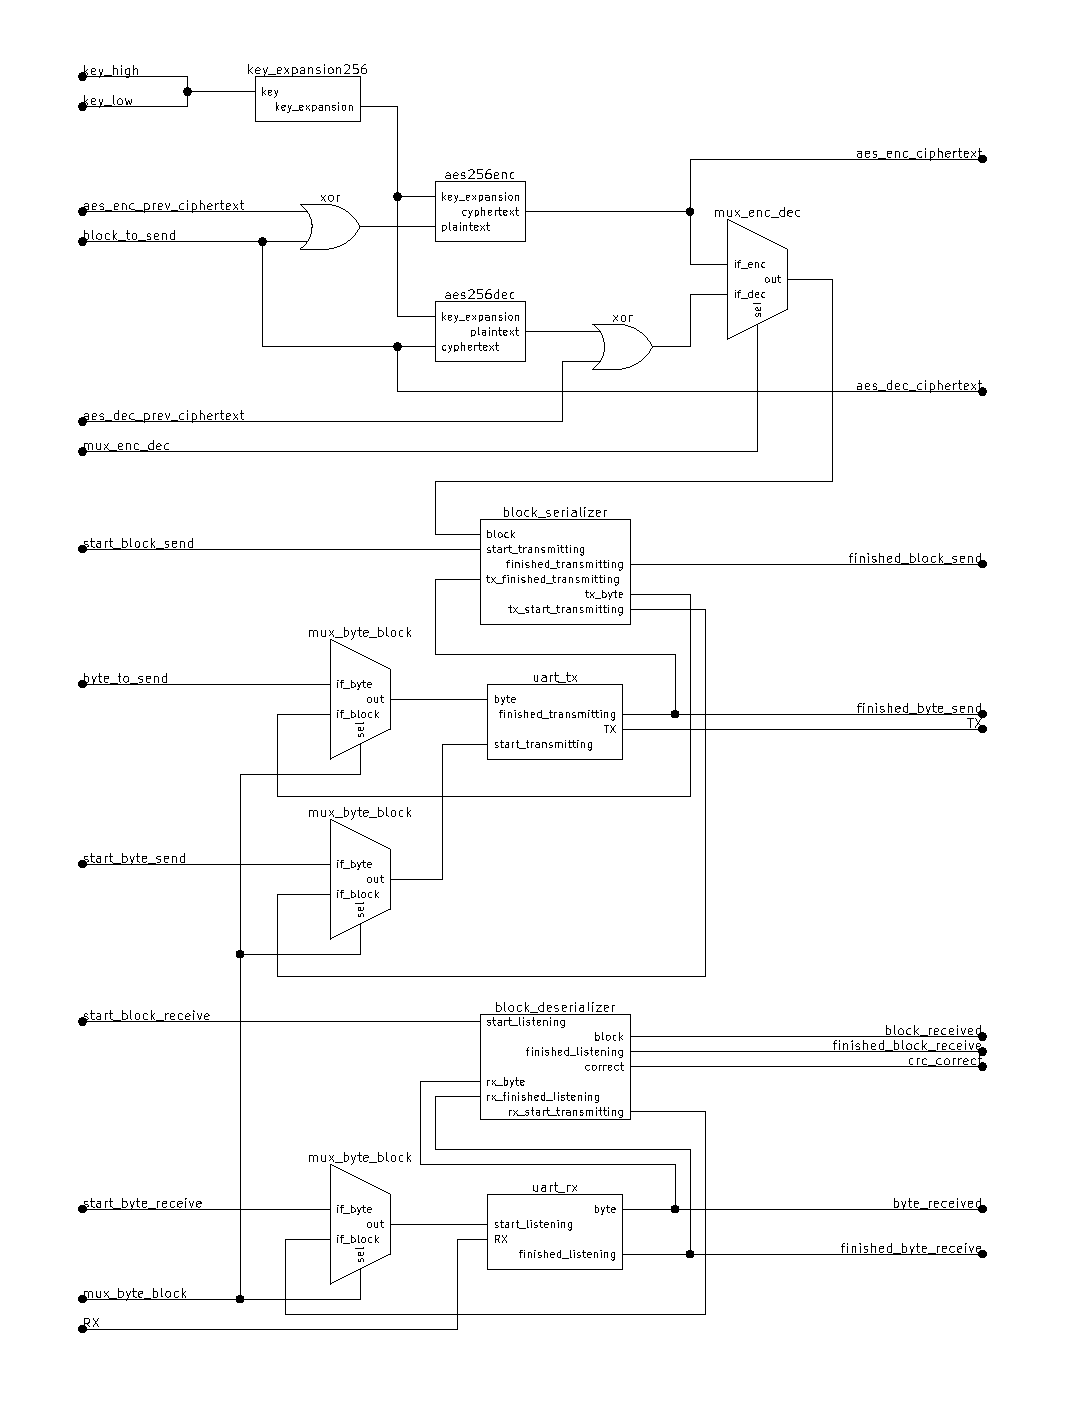
\includegraphics{pictures/communicator.pdf}
\caption{Schemat modułu \textit{communicator}}
\label{fig:communicator-schemat}
\end{figure}

%%%%%%%%%%%%%%%%%%%%%%%%%%%%%%%%%%%%%%%%%%%%%%%%%%%%%%%%%%%%%%%%%%%%%%%%%%%%%%%%%%%%%%%%%%%%%%%%%%%%%%%%
%%%%%%%%%%%%%%%%%%%%%%%%%%%%%%%%%%%%%%%%%%%%%%%%%%%%%%%%%%%%%%%%%%%%%%%%%%%%%%%%%%%%%%%%%%%%%%%%%%%%%%%%
%%%%%%%%%%%%%%%%%%%%%%%%%%%%%%%%%%%%%%%%%%%%%%%%%%%%%%%%%%%%%%%%%%%%%%%%%%%%%%%%%%%%%%%%%%%%%%%%%%%%%%%%


% \newpage
\subsection{Skrypt klienta}
Skrypt klienta jest implementacją algorytmu komunikacji z serwerem szyfrującym (płytką Terasic DE1-SOC) przedstawionego w sekcji \ref{sec:przebieg-komunikacji}. Program przyjmuje od użytkownika tryb działania (szyfrowanie lub deszyfrowanie), klucz szyfrowania, wektor inicjalizacji oraz nazwy plików wejściowego i wyjściowego. Program odczytuje z dysku dane wejściowe, wysyła je do serwera oraz odbiera dane przetworzone i zapisuje je do pliku wynikowego. Jest napisany w języku python, oraz korzysta z bibliotek:
\begin{description}[noitemsep]
\item[serial] -- komunikacja przez port szeregowy UART
\item[threading] -- wielowątkowość związana z jednoczesnym wysyłaniem i odbieraniem bloków
\item[crcmod] -- obliczanie sumy kontrolnej crc16
\item[struct] -- konwersja liczby crc16 do tablicy bajtów możliwej do przesłania biblioteką serial
\item[argparse] -- parsowanie argumentów programu
\item[re] -- obsługa wyrażeń regularnych
\end{description}

\subsubsection{Padding}
Algorytm AES działa na blokach o wielkości 128b. W celu przetwarzania danych o wielkości nie będącej wielokrotnością rozmiaru bloku stosowany jest padding. W tym projekcie należy to do zadań klienta. Używany jest padding metodą dopełniania bloków do rozmiarów 128b bajtami o wartości równej brakującej liczbie bajtów. W celu uniknięcia niejednoznaczności przy usuwaniu wypełnienia, do wiadomości o wielkości będącej wielokrotnością 128b dodawany jest cały blok bajtów o wartości 16. W ten sposób ostatni bajt wiadomości zawsze zawiera liczbę bajtów dopełnienia, co pozwala na jednoznaczne usunięcie paddingu. 

Zastosowana metoda jest jedną ze standardowych praktyk. Została wybrana ze względu na fakt, że jest używana przez program \textit{openssl}, z którym produkt końcowy ma być kompatybilny. Jest zaimplementowana w sposób zgodny ze standardem RFC-2315 \cite{padding-rfc}.





\newpage